\documentclass[a4paper,11pt]{article}

%LAYOUT
\usepackage[section]{placeins}
\usepackage{pdfpages}
\usepackage{wrapfig}
\usepackage{subcaption}
\usepackage{makecell}
\usepackage{geometry}
\usepackage{float}

%MATH
\usepackage{amsmath}
\usepackage{amsfonts}
\usepackage{amssymb}
\usepackage{graphicx}
%\usepackage{equation}{section} %Resets equation numbering within each section
\usepackage{esint}
\usepackage{multirow}
\usepackage{bigdelim}
\usepackage{cancel}

%LANGUAGE
%\usepackage[T1]{fontenc}
\usepackage[utf8x]{inputenc}
\usepackage[swedish, english]{babel} %Last language chosen as active
\usepackage[colorlinks=true, linkcolor=blue]{hyperref}
\usepackage[font=small,labelfont=bf, margin=.6cm]{caption}
\hypersetup{citecolor=cyan}

%PROGRAMMING
\usepackage{listings} % Allows to input code with the command \lstinputlisting{helloworld.c}
%Also use \lstset{language=C, numbers=left, breaklines=true} to highlight C keywords, show line numbers on the left and to automatically break lines that are too long (still keeps numbering correct).
\usepackage{enumerate}
\usepackage{tikz}

%BIBLIOGRAPHY AND NOTES
\usepackage{endnotes}
%\usepackage{harvard}
\usepackage{cite}
\usepackage{natbib}

%To enter bibliography, do
%\clearpage
%\bibliography{BibName.bib}

%\cite{ref} for citations

%\usepackage{pdfpages} %To insert external pdfs

\begin{document}
\title{Modeling of current-reinforced random walks}
\author{David J\"{a}derberg, Kristoffer Jonsson}
\maketitle

\section*{Abstract}
\label{sec:abstract}

The occurrence of reinforced random walks are present in many complex systems, everything from biological systems such as construction of blood vessels or neural networks to trail-laying ants can at some level be described by a reinforced random walk. Modelling complex systems with reinforced random walks is often done by simulating particles travelling from node to node in a specified graph, constructing networks where the paths taken by the particles depend on local environmental parameters in each node.

Results of simulating such systems show that the characteristics of the constructed network and the time needed until a solution is found strongly depend on the path maintenance parameter, $\mu$, as well as the number of sources versus the number of sinks and their geographical placement. If in the linear state, i.e.\@ $\mu = 1$, the network will consist of the shortest paths from each source to each sink and it takes a long time to find a solution. If in the non-linear state, i.e.\@ $\mu > 1$, there is instead a preference to share paths rather than taking the shortest path and the time needed to find a solution is much smaller. Results also show that if the value of $\mu$ is increased enough the simulation breaks down and the solution found does not represent any network at all. 

The model is also tested on a graph over the street network of the Uppsala, Sweden, where source are placed in the residential areas and sinks are placed in the city center. This can be seen as a simulation of traffic flow during rush hours and used to understand how to deal with traffic congestion.

The implementation is done in \texttt{C++} with the library OpenMP for parallelism. In order to get better performance the nodes are numbered and ordered with graph partitioning schemes. Measurements of speedup and sizeup show that the parallel implementation significantly increase performance. 
\pagebreak
\tableofcontents
\pagebreak
\section{Introduction}
\label{sec:introduction}
Networks created by reinforced random walks are found in many complex systems, everything from biological systems such as construction of blood vessels or neural networks to trail-laying ants can at some level be described by a reinforced random walk. These biological systems can be seen as a massive cluster of tiny computational units, e.g.\@ ants, generating the network in parallel, with every tiny component only knowing its local environment. Modelling complex systems with reinforced random walks is often done by simulating particles traveling from node to node in a specified graph, constructing networks. The paths taken by the particles depend on local environmental parameters in each node. The parameters for a node can for example be the particle density within the node or the flow of particles to another node. The probability for a particle to move to another node then depend on these parameters. Ants for example, as presented in \cite{Schweitzer1997153}, move around in their search for food or building material drop pheromone in certain patterns. If an ant has found food it drops an amount of pheromone which other ants can then register. Ants want to move along paths where the pheromone concentration is high, i.e.\@ where other ants are moving. This causes the ants to create so called current-reinforced patterns through their transport network.

Previous studies have shown how biological systems can be modelled by current-reinforced random walks. In current-reinforced random walks, the probability for a particle to move to another node depends on the flow of particles to that node, i.e.\@ the current of particles. The basic idea of a current-reinforced random walk is to find the shortest path between a source and a sink for a given graph. This optimises the path length for each individual path from the sources to the sinks. The algorithm for network creation by current-reinforced random walks used in \cite{Sumpter} converges to the shortest path through the graph \cite{Ito}. When utilising non linear current-reinforced random walks a combination of path length and path maintenance is minimised. For example, ants may want to construct one big road rather than many small ones to easier keep needles and dirt off the road while not making each individual path that much longer. The actual function that is minimised in non linear cases is not yet known, a suggestion for this function is given in \cite{Sumpter}.

Another example of where to find networks that can be modelled by current-reinforced random walks is in certain types of electrical systems. As presented in \cite{Sumpter}, the movement of the electrons in special types of current dependent conductors can be modelled by current-reinforced random walks. In these systems the conductivity in the conductors is proportional to the amount of electrons flowing through it, i.e.\@ the current. This property enables the analogy to ant trail networks where pheromone concentration corresponds to the conductivity in the electrical network. What is unanimous for all these different networks is that the particles flowing within the network have no global information of the network itself, i.e.\@ they can only know and affect their local environment. 

When simulating these systems It may seem natural to implement the algorithms within a parallel setting due to the parallel nature of the systems themselves. However, previous simulations of current-reinforced random walks have been implemented serially in low performance environments \cite{Sumpter, Ma2012rib}. This is mainly because high performance parallel programming is not that simple as it may seem at first glance. Since all particles affect and react to their local environment synchronisation is needed when moving particles around in the network, otherwise the computation would be corrupted. This project aims to be the first high performance parallel implementation of the current-reinforced random walk network creation presented in \cite{Sumpter}, utilising high performance languages such as \texttt{C++} along with graph partitioning schemes such as METIS \cite{Lasalle} for better performance. The purpose is to decrease computation time and increase the problem size. Relevant measures for this is speedup and sizeup as a function of number of utilised parallel cores.
\section{Theory}
\label{sec:theory}

\subsection{Mathematical modeling}
The theory behind the mathematical modeling is very much based upon the modeling described in Section 3 in the paper \cite{Current}. The basic idea of a current-reinforced random walk is to find the shortest path through a given graph. The core of this modeling is that there are sources, sinks, nodes, particles and edges all organized within a graph representing a network. The fundamental idea is that sources send out information, sinks want information and particles represent information. Edges are connections between sources, sinks and nodes and represent a path for the information to spread. Sources have a production rate, i.e the rate at which new particles are being injected into the system. Sinks have a removal rate, i.e. the rate at which particles are being removed from the system. Sources, sinks and nodes can all contain particles. For a system to have a viable solution for a shortest path between sources and sinks the cumulative production rate of all the sources must be less than or equal to the cumulative removal rate of all the sinks, otherwise no flow equilibrium can be established.

There are several analogies in nature to this modeling. For example, the transport network of many pheromone dropping ants can be modeled by current-reinforced random walks as presented in \cite{Schweitzer1997153}. When the ants move around in their search for food or building material they drop pheromone in certain patterns. If an ant has found food it drops an amount of pheromone which other ants then can register. Ants want to move along paths where other ants are moving, and are more likely to do so if there is a high pheromone concentration. This causes the ants to create current-reinforced patterns through their transport network.

An other example is how the current and conductivity changes in special electrical networks as presented in \cite{Doyle}. Here the conductivity changes with the current. This causes electrons to more easily flow where there already is a current present, leading to shortest path patterns through the electrical network. 

There are some necessary parameters for this model to make sense. These parameters and their analogy in both electrical networks and ant trail networks are shown in Table \ref{tab:parameters}.
\begin{table}
\centering
\caption{Table shows the necessary parameters for the current-reinforced random walk modeling and their analogy in electrical networks and ant trail networks. $i$ denotes that the parameter corresponds to node $i$ and $ij$ denotes that the parameter corresponds to the edge between node $i$ and node $j$.}
\label{tab:parameters}
\begin{tabular}{ c | c | c }                       
	\textbf{Parameter} & \textbf{Electrical network} & \textbf{Ant trails} \\
	\hline
	$l_{ij}$ & length in space & length in space \\
	\hline
	$N_{i}$ & potential & number of ants \\
	\hline
	$I_{ij}$ & current & flow of ants \\
	\hline
	$D_{ij}$ & conductivity & pheromone concentration \\
	\hline
	$C_{i}$ & capacitance & total pheromone density \\
	\hline
	$q$ & reinforcement intensity & pheromone drop rate \\
	\hline
	$\lambda$ & conductivity decrease rate & pheromone evaporation rate \\
\end{tabular} 
\end{table}

The probability for a particle to move to another node in this particular current-reinforced random walk depends on the flow of particles to that node, i.e. the current of particles. This optimizes the path length for each individual path from the sources to the sinks, i.e it minimizes 

\begin{equation}
\sum_{j \in \text{Neighbors}(i)} l_{ij} \bar{I}_{ij},
\end{equation}

\noindent where $l_{ij}$ is the edge length between node $i$ and $j$ and $\bar{I}_{ij}$ is the corresponding mean flow of particles. When utilizing non linear current-reinforced random walks a combination of path length and path maintenance is optimized. 

Non linear current-reinforced random walks describe many networks created by animals. Ants for example may want to construct one big road for transporting food rather than many small ones to easier keep needles and dirt off the road while not making each individual path that much longer.


\subsubsection{Preparation}
The preparation begins with each node calculating the mean flow to each of its neighbors as
\begin{equation}
\bar{I}_{ij} = \frac{(N_i - N_j)D_{ij}}{l_{ij}},
\end{equation}
from which it can be seen that the mean flow depends on the conductivity of each edge, $D_{ij}$, which is 	initialized at and kept at or above some minimal value.
The actual flow along the edge $ij$ can then be found as
\begin{equation}
I_{ij} = \text{Poi}(|\bar{I}_{ij}|\Delta t).
\end{equation}
In terms of implementation, it is important that nodes that are connected to the same edge agree on the same number of particles to transfer. This is ensured by allowing only the node with a larger number of particles to randomize the value and then both nodes use that value when updating the number of particles. This work is done at the node with the largest number of particles, since it is also important to ensure that there are never fewer than zero particles at a node and the number of particles will be decreasing at the node with the largest number of particles. When a node has a smaller number of particles than a given neighbor, the node always calculates the flow to that neighbor as zero. After all nodes have calculated and stored $\bar{I}$ and $I$, the preparation step is finished.

\subsubsection{Confirmation}
At the beginning of the confirmation part, all the data regarding how many particles will move along each edge is available. And so each node begins by updating the number of particles that is has as
 \begin{equation}
 N_i(t + \Delta t) = N_i(t) + \sum_{j \in \text{Neighbors}(i)} \left( I_{ji} - I_{ij} \right)
 \end{equation}
 The flow should theoretically be symmetric, but since only one particle has randomized a value, and the other has set it to zero, the flow is not symmetric in this implementation.
 
After that, the final part of the step begins, in which several parameters that are relevant to the algorithm are updated. First is the conductivity, which can be calculated as
\begin{equation}
D_{ij}(t + \Delta t) = D_{ij}(t) + q|\bar{I}|^\mu - \lambda D_{ij}(t)\Delta t,
\end{equation}

where $q$ is the reinforcement intensity caused by per unit flow, $\mu$ is the path maintenance parameter, $\lambda$ is the conductivity decay parameter and $\Delta t$ is the time step. If $\mu$ is set to one the current-reinforced random walk is linear and will converge to the same solution every time. If on the other hand $\mu$ is set to greater than one the current-reinforced random walk becomes non-linear and will not converge to the same solution every time that a system is simulated. 

Next to be calculated is the capacitance, which is calculated as 
 \begin{equation}
 C_i = \sum_{j \in \text{Neighbors}(i)} D_{ij}
 \end{equation}
 and finally the potential is calculated as
 \begin{equation}
 P_i = \frac{N_i}{C_i}.
 \end{equation}
 
 \noindent When this is done the step is finished and the next step can be started.
 
 \subsection{Implementation and parallelism}
\section{Result}
\label{sec:result}

\subsection{Homogeneous grid}

A homogenous grid where each node has been perturbed a small amount was used to execute the algorithm with several different choices of parameters, with a focus on the maintenance parameter, $\mu$. This is shown in fig. (\ref{fig:homogeneous}), which shows that when $\mu = 1$, i.e. the linear case, the solution that is found is the shortest path between each source and sink. When $\mu > 1$, the path chosen may not be the shortest path and there also exists a preference to share paths.

\begin{figure}
\centering
\begin{subfigure}[b]{0.48\textwidth}
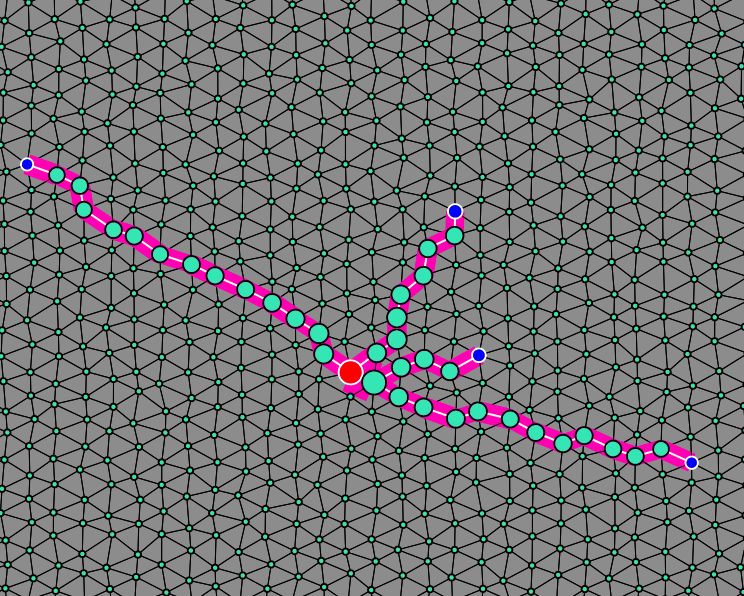
\includegraphics[width=\textwidth]{/Users/david/Dropbox/Project/presentation/Lin.png}
\caption{The simulated solution when $\mu=1$. This is the shortest possible path from the source to each sink.
\\
\\}
\end{subfigure}
~
\begin{subfigure}[b]{0.48\textwidth}
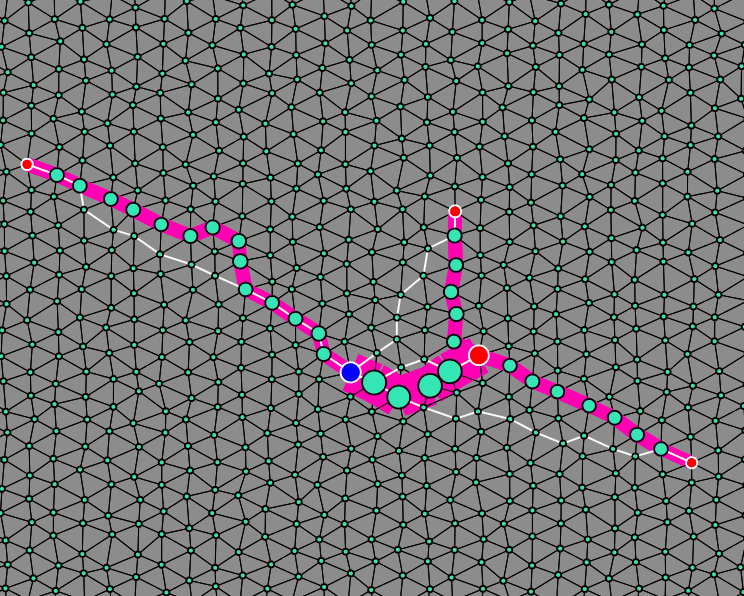
\includegraphics[width=\textwidth]{/Users/david/Dropbox/Project/presentation/NonLin.png}
\caption{The simulated solution when $\mu=1.5$. This is not the shortest possible path, but rather shows a preference to take the same path as other particles, if it is not too much longer.}
\end{subfigure}
\caption{Figure shows the solutions found by the simulation on a nearly homogenous grid. The pink lines show the flow along each edge, with the thickness of the line showing the amount of flow. The shortest path from each source to each sinks has been marked with a thin white line. The parameters used are $q = 10^{-4},\lambda = 10^{-3},$ and $D_{min}=5 \cdot 10^{-2}$. Each source (red) produces 1000 particles each time unit and all sinks (blue) can together remove as many particles as are produced each time unit (evenly divided between the sinks).}
\label{fig:homogeneous}
\end{figure}

\subsection{City}

Another grid was created using road data from the city of Uppsala, Sweden.

\subsection{Parallelism}

\section{Conclusion}
\label{sec:conslusion}


\clearpage
\bibliographystyle{unsrt}
\bibliography{ref}

\clearpage
\section{Appendix}
\label{sec:appendix}

\subsection{Object oriented programming}

There are two main class structures used in the program, one to represent graphs and one to represent different computational methods.

The class \texttt{NodeSet} exists to model a graph. This is done by storing all nodes, each in an instance of the class \texttt{Node}, and their neighbors, where each \texttt{Node} has a list of pointers to all its neighbors. To model sources and sinks, the classes \texttt{Source} and \texttt{Sink} exists, and they are both subclasses of \texttt{Node}. This is in itself enough to model a graph, but there are also some extensions to help dealing with graphs where every node has a given position in a Euclidean space. To do this, the classes \texttt{PositionedNodeSet}, \texttt{PositionedNode}, \texttt{PositionedSource}, and \texttt{PositionedSink} are introduced, which are all similar to their non-positioned versions. These classes are then used as tools when implementing the actual computations.

The class structure allows to implement different computation algorithms using the same framework. To do this, there exists the abstract class \texttt{Algorithm}, which contains a few pure virtual methods that must be implemented by each subclass. The main subclass of \texttt{Algorithm} is \texttt{CurrentWalk}, which implements the current-reinforced random walks. Each instance of \texttt{Algorithm} expects to be given a single \texttt{Node} and uses that as the basis for its calculations.

These two groups of classes are then used by the main program to perform simulations. Given a method to create instances of some subclass of \texttt{Algorithm}, the main program is then able to construct a \texttt{NodeSet} with a set of \texttt{Node}s and an \texttt{Algorithm} for each \texttt{Node}. The algorithm advances using the \texttt{takeStep()} method in \texttt{NodeSet}. A schematic overview of this structure is shown in Figure. (\ref{fig:graphToClass}).

\begin{figure}[H]
\centering
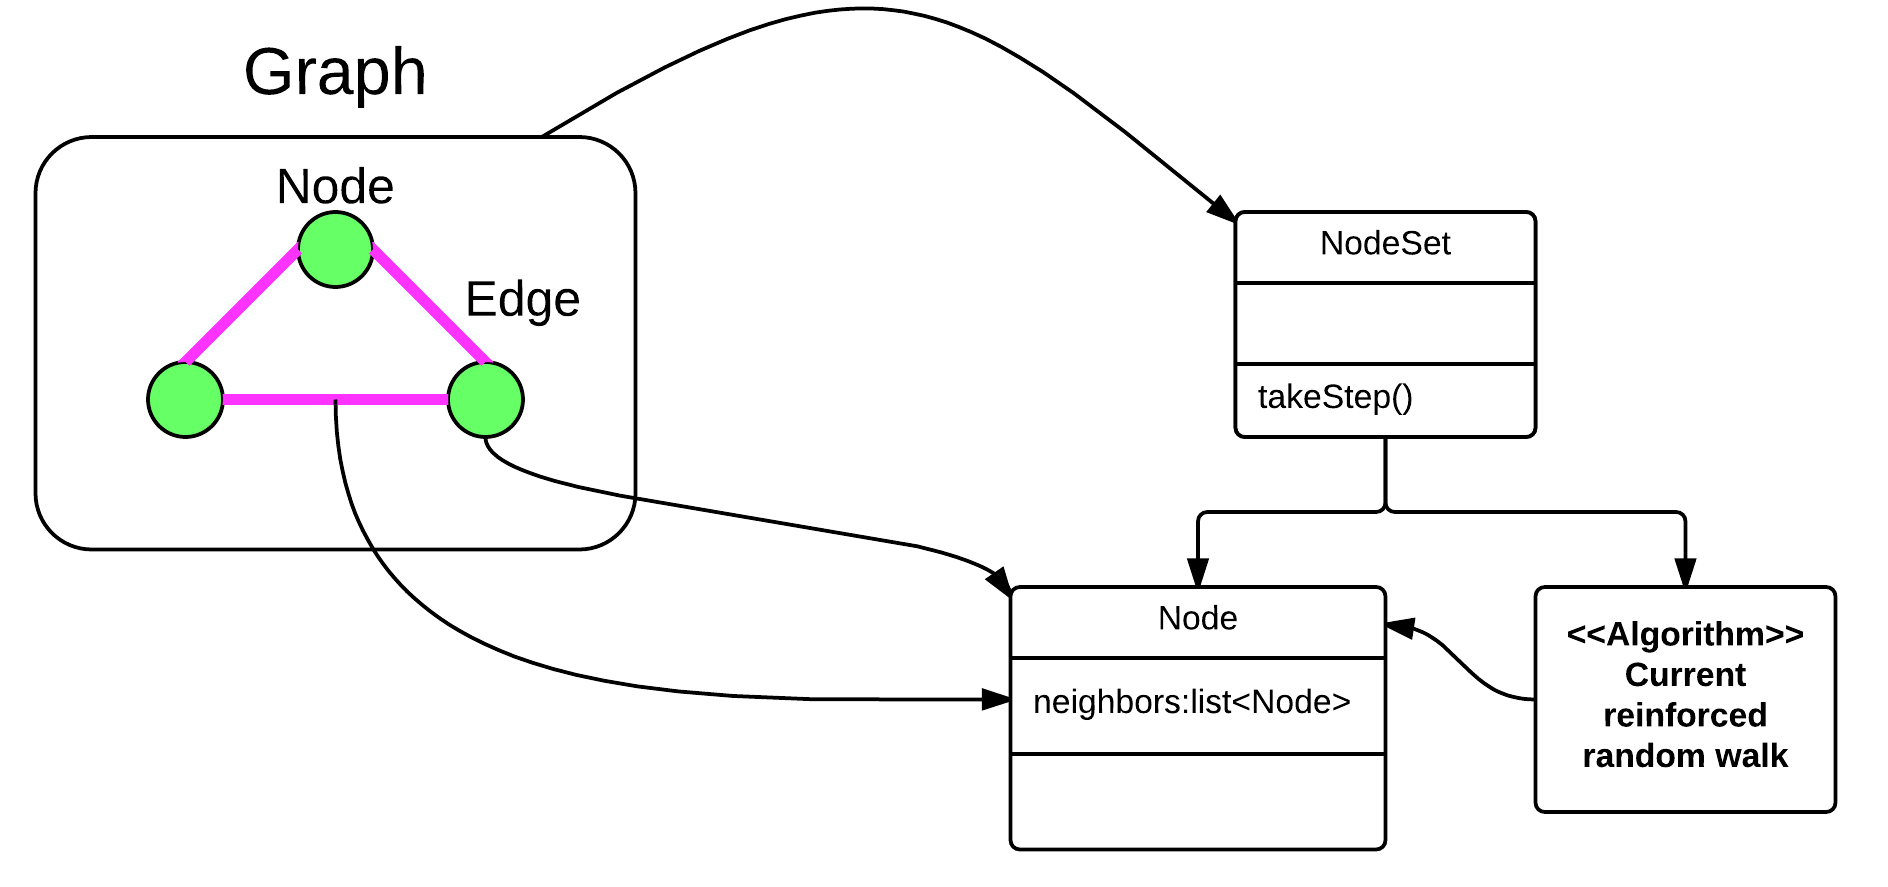
\includegraphics[width=0.95\textwidth]{img/graphToClass.png}
\caption{An overview of the relation between elements in the graph and different classes in the program structure. It can be seen that each \texttt{NodeSet} contains both a set of \texttt{Node}s and a set of \texttt{Algorithm}s.}
\label{fig:graphToClass}
\end{figure}

\subsection{Metis and parallelism}

%\subsection{Algorithm}
%\label{sec:appendix:algorithm}
%The probability for a particle to move to another node in this particular current-reinforced random walk depends on the flow of particles to that node, i.e. the current of particles. This optimizes the path length for each individual path from the sources to the sinks, i.e it minimizes 
%
%\begin{equation}
%\sum_{j \in \text{Neighbors}(i)} l_{ij} \bar{I}_{ij},
%\end{equation}
%
%\noindent where $l_{ij}$ is the edge length between node $i$ and $j$ and $\bar{I}_{ij}$ is the corresponding mean flow of particles. When utilizing non linear current-reinforced random walks a combination of path length and path maintenance is optimized. 
%
%There are some necessary parameters for this model to make sense. These parameters and their analogy in both electrical networks and ant trail networks are shown in Table \ref{tab:parameters}.
%
%\begin{table}
%\centering
%\caption{Table shows the necessary parameters for the current-reinforced random walk modeling and their analogy in electrical networks and ant trail networks. $i$ denotes that the parameter corresponds to node $i$ and $ij$ denotes that the parameter corresponds to the edge between node $i$ and node $j$.}
%\label{tab:parameters}
%\begin{tabular}{ c | c | c }                       
%	\textbf{Parameter} & \textbf{Electrical network} & \textbf{Ant trails} \\
%	\hline
%	$l_{ij}$ & length in space & length in space \\
%	\hline
%	$N_{i}$ & number of electrons & number of ants \\
%	\hline	
%	$P_{i}$ & potential & inverse flowness \\
%	\hline
%	$I_{ij}$ & current & flow of ants \\
%	\hline
%	$D_{ij}$ & conductivity & pheromone concentration \\
%	\hline
%	$C_{i}$ & capacitance & total pheromone density \\
%	\hline
%	$q$ & reinforcement intensity & pheromone drop rate \\
%	\hline
%	$\lambda$ & conductivity decrease rate & pheromone evaporation rate \\
%\end{tabular} 
%\end{table}
%
%\subsubsection{Preparation}
%The preparation begins with each node calculating the mean flow to each of its neighbors as
%\begin{equation}
%\bar{I}_{ij} = \frac{(N_i - N_j)D_{ij}}{l_{ij}},
%\end{equation}
%from which it can be seen that the mean flow depends on the conductivity of each edge, $D_{ij}$, which is 	initialized at and kept at or above some minimal value.
%The actual flow along the edge $ij$ can then be found as
%\begin{equation}
%I_{ij} = \text{Poi}(|\bar{I}_{ij}|\Delta t).
%\end{equation}
%In terms of implementation, it is important that nodes that are connected to the same edge agree on the same number of particles to transfer. This is ensured by allowing only the node with a larger number of particles to randomize the value and then both nodes use that value when updating the number of particles. This work is done at the node with the largest number of particles, since it is also important to ensure that there are never fewer than zero particles at a node and the number of particles will be decreasing at the node with the largest number of particles. When a node has a smaller number of particles than a given neighbor, the node always calculates the flow to that neighbor as zero. After all nodes have calculated and stored $\bar{I}$ and $I$, the preparation step is finished.
%
%\subsubsection{Confirmation}
%At the beginning of the confirmation part, all the data regarding how many particles will move along each edge is available. And so each node begins by updating the number of particles that is has as
% \begin{equation}
% N_i(t + \Delta t) = N_i(t) + \sum_{j \in \text{Neighbors}(i)} \left( I_{ji} - I_{ij} \right)
% \end{equation}
% The flow should theoretically be symmetric, but since only one particle has randomized a value, and the other has set it to zero, the flow is not symmetric in this implementation.
% 
%After that, the final part of the step begins, in which several parameters that are relevant to the algorithm are updated. First is the conductivity, which can be calculated as
%\begin{equation}
%D_{ij}(t + \Delta t) = D_{ij}(t) + q|\bar{I}|^\mu - \lambda D_{ij}(t)\Delta t,
%\end{equation}
%
%where $q$ is the reinforcement intensity caused by per unit flow, $\mu$ is the path maintenance parameter, $\lambda$ is the conductivity decay parameter and $\Delta t$ is the time step. If $\mu$ is set to one the current-reinforced random walk is linear and will converge to the same solution every time. If on the other hand $\mu$ is set to greater than one the current-reinforced random walk becomes non-linear and will not converge to the same solution every time that a system is simulated. 
%
%Next to be calculated is the capacitance, which is calculated as 
% \begin{equation}
% C_i = \sum_{j \in \text{Neighbors}(i)} D_{ij}
% \end{equation}
% and finally the potential is calculated as
% \begin{equation}
% P_i = \frac{N_i}{C_i}.
% \end{equation}
% 
% \noindent When this is done the step is finished and the next step can be started.

\end{document}







